%!TEX root = <main.tex>
%\chapter{Revisão Bibliográfica}
\chapter{Modelagem e Controle Cinemático}
Neste capitulo serão abordados os conceitos necessários para modelagem e controle de manipuladores robóticos, focando no que foi utilizado nesse projeto, para implementação no manipulador 4-DOF chamado de TETIS. Os tópicos tratados aqui podem ser encontrados em \citep{siciliano, petercorke}.

\section{Cinemática Direta}
Um manipulador robótico é composto de uma série de corpos rígidos denominados \textit{elos} conectados através de \textit{juntas}. 
Juntas podem ser:
\begin{itemize} 
\item Revolução
\item Prismática
\end{itemize}

Essa estrutura é chamada de cadeia cinemática.
Um extremo da cadeia é fixado a base e o outro ao efetuador.
Nesse texto serão abordadas apenas cadeias cinemáticas abertas, ou seja, aquelas em que existe apenas uma sequência de elos conectando os dois extremos da cadeia.
Cada junta acrescenta um grau de liberdade (DOF), ao qual está associado a uma variável de junta. No caso de uma junta de revolução um ângulo e no caso de uma junta prismática um deslocamento.
O objetivo da cinemática direta é calcular a posição e orientação do efetuador em função das variáveis das juntas.

%É possível expressar a 

Uma cadeia cinemática aberta é constituída por $n+1$ elos numerados de $0$ a $n$, onde o Elo 0 é fixado a base por convenção. O método utilizado consiste em definir um sistema de coordenadas associado a cada elo e calcular a transformação homogênea entre elos consecutivos. Em seguida a transformação do n-ésimo sistema de coordenadas pode ser obtida de forma recursiva como
\begin{equation}\label{eq:cinedireta}
\bm{T}_{0n}(\bm{q}) = \bm{T}_{01}(q_1) \bm{T}_{12}(q_{2}) {\dots} \bm{T}_{n-1,n}(q_n)
\end{equation}
onde $\bm{T}_{i-1,i}(q_i)$ denota a transformação homogênea do sistema de coordenadas solidário ao elo $i-1$ àquele solidário ao elo $i$.

Logo a transformação homogênea do efetuador final com respeito a base é dada por
\begin{equation} \label{eq:base_efetuador}
\bm{T}_{be}({q}) = {T}_{b0} {T}_{0n}({q}) {T}_{ne} 
\end{equation}

\subsection{Convenção Denavit-Hartenberg} \label{sec:denavit}
Para calcular a cinemática direta para uma manipulador de cadeia cinemática aberta de acordo com a equação \eqref{eq:cinedireta} um método sistemático foi definido para obter a relação entre a posição e orientação de dois elos consecutivos. A convenção Denavit-Hartenberg especifica um conjunto de regras sobre como definir os sistemas de coordenadas de cada elo.

Seja o Eixo $i$ o eixo da junta que conecta o elo $i-1$, ao elo $i$, então:

\begin{itemize}
\item Escolher o eixo $z_i$ ao longo do eixo da junta $i+1$.
\item Colocar a origem $O_i$ na interseção do eixo $z_i$ com a normal comum entre os eixos $z_{i-1}$ e $z_i$
\item Escolher $x_i$ ao longo da normal comum aos eixos $z_{i-1}$ e $z_i$, com direção da junta $i$ para a junta $i+1$. 
\item O eixo $y_i = z_i \times x_i$ é escolhido de forma a completar o sistema de coordenadas.
\end{itemize}

Essa convenção resulta em uma definição não única do sistema de coordenadas nos seguintes casos:

\begin{itemize}
\item Para o sistema de coordenadas $0$, somente a direção do eixo $z_0$ é especificada, portanto a escolha de $O_0$ e $ x_0$ é arbitrária.
\item Para o sistema de coordenadas $n$, como não existe junta $n+1$, $z_n$ não está definido, mas $x_n$ deve ser normal ao eixo $z_{n-1}$. Tipicamente escolhe-se $z_n$ alinhado com $z_{n-1}$.
\item Quando dois eixos consecutivos são paralelos, a normal comum entre eles não é definida de forma única. Tipicamente escolhe-se $O_i$ na junta $i+1$
\item  Quando dois eixos consecutivos se interceptam, direção de $x_i$ é normal e o sentido é arbitrário. Escolhe-se $O_i$ na intersecção.
\item Quando a junta $i$ é prismática a direção de $z_{i-1}$ é arbitrária.
\end{itemize}

Após determinados os sistemas de coordenadas, é possível determinar a posição e orientação de um referencial em relação ao outro através dos seguintes parâmetros:
\begin{itemize}
\item $a_i$ distância entre $z_{i-1}$ e $z_i$ ao longo de $x_i$
\item $\alpha_i$ ângulo entre $z_{i-1}$ e $z_i$ ao redor de $x_i$
\item $d_i$ distância entre $x_{i-1}$ e $x_i$ ao longo de $z_{i-1}$
\item $\theta_i$ ângulo entre $x_{i-1}$ e $x_i$ ao redor de $z_{i-1}$
\end{itemize}
\subsection{Espaço das Juntas e Espaço Operacional}
Para que o efetuador final de um manipulador realize alguma tarefa é necessário atribuir uma posição e orientação desejada, que  pode ser função do tempo (trajetória). Surge então o problema de representar posição e orientação. 

Para descrever a posição utiliza-se as coordenadas cartesianas. Para a orientação adota-se uma representação mínima (ângulos de Euler), descrevendo a rotação do efetuador em relação ao sistema de coordenadas da base. Portanto é possível descrever a \textit{pose} do efetuador através do vetor
\begin{equation} \label{eq:op_space}
\bm{x}_e = \m{ \bm{p}_e \\ \bm{\phi}_e}
\end{equation}
onde $\bm{p}_e$ descreve a posição e $\bm{\phi}_e$ a orientação.

O \textit{espaço das juntas} denota o espaço em que o vetor $(n \times 1)$ das variáveis das juntas
\begin{equation} \label{eq:joint_space}
\bm{q} = \m{q_1 \\ \vdots \\ q_n}
\end{equation} 
é definido. Se a junta é de revolução utiliza-se $q_i = \theta_i$, se é prismática $q_i = d_i$.

\section{Cinemática Diferencial}
%\subsection{Jacobiano Geométrico}
%TODO
\subsection{Jacobiano Analítico}
Quando a posição e orientação do efetuador são dadas em função de um número mínimos de parâmetros no espaço operacional é possível computar o Jacobiano pela diferenciação das equações da cinemática direta em função das variáveis das juntas.
Para isso utiliza-se a técnica analítica.

Seja $\bm{p}_e$ a posição do sistema de coordenadas do efetuador representada no sistema de coordenadas da base. O vetor $\dot{\bm{p}}_e$ é portanto a velocidade de translação, ou linear.
\begin{equation} \label{eq:jacob_pos}
\dot{\bm{p}}_e = \frac{\partial \bm{p}_e }{\partial \bm{q}} \dot{\bm{q}} = \bm{J}_P (\bm{q}) \dot{\bm{q}} 
\end{equation}

Para a velocidade angular, pode ser considerada uma representação mínima da orientação em função de três variáveis $\phi_e$. 
A derivada no tempo $\dot{\bm{\phi}}_e$ não é igual a velocidade angular, no entanto, conhecida a função $\bm{\phi}_e(\bm{q})$:

\begin{equation} \label{eq:jacob_or}
\dot{\bm{\phi}}_e = \frac{\partial \bm{\phi}_e}{\partial \bm{q}} \bm{\dot{q}} = \bm{J}_{\phi}(\bm{q})\bm{\dot{q}}
\end{equation}

Sob essas premissas a cinemática diferencial pode ser obtida como:
\begin{equation} \label{eq:jacoba}
\bm{\dot{x}}_e = \m{\bm{\dot{p}}_e \\ \bm{\dot{\phi}}_e} = \m{\bm{J}_P(\bm{q}) \\ \bm{J_\phi}(\bm{q})} \bm{\dot{q}} = \bm{J}_A (\bm{q}) \dot{\bm{q}}
\end{equation}

 
\section{Controle Cinemático} \label{sec:controle_cinematico}
O estratégia de controle cinemático pode ser aplicada quando considera-se que a dinâmica do manipulador pode ser desprezada. Essa hipótese se sustenta quando as seguintes premissas são válidas:
\begin{itemize}
\item Elevados fatores de redução nas juntas.
\item Baixas velocidades na realização das tarefas.
\item Existência uma malha de controle de velocidade de alto desempenho em cada junta.
\end{itemize}

A maioria dos manipuladores possui uma malha de controle de velocidade em nível de juntas como na figura \ref{fig:controlejuntas}. Logo, para um controle de alto ganho temos que:
\[ \bm{u} \approx \dot{\bm{q}}\]

\begin{figure}[h!]
\centering
\begin{tikzpicture}[auto, node distance=2cm,>=latex']
    % We start by placing the blocks
    \node [input, name=input] {};
    \node [sum, right of=input] (sum) {};
    \node [block, right of=sum] (K) {$K$};
    \node [block, right of=K] (PWM) {PWM};
    \node [block, right of=PWM] (Robo) {Robô};
    \node [block, right of=Robo] (JA) {$\bm{J}_A$};
    \node [block, right of=JA] (Integral) {$\int$};
    \node [tmp, below of=K] (tmp1){};
    \node [output, right of=Integral] (output) {};

    % Once the nodes are placed, connecting them is easy. 
    \draw [draw,->] (input) -- node {$u$} (sum);
    \draw [->] (sum) -- node {$e$} (K);
    \draw [->] (K) -- node {$v$} (PWM);
    \draw [->] (PWM) -- node [name=tau] {$\tau$} (Robo);
    \draw [->] (Robo) -- node [name=dtheta] {$\dot{q}$} (JA);
    \draw [->] (JA) -- node {$\dot{x}$} (Integral);
    \draw [->] (Integral) -- node [name=x] {$x$}(output);
    \draw [->] (dtheta) |- (tmp1)-| node[pos=0.99] {$-$} (sum);
\end{tikzpicture}
\caption{Diagrama de Blocos: Malha de Controle de Velocidade a nível de juntas.}
\label{fig:controlejuntas}
\end{figure}


Portanto é possível implementar o controle cinemático segundo o diagrama \ref{fig:controlecinematico} 	

\begin{figure}[h!]
\centering
\begin{tikzpicture}[auto, node distance=2cm,>=latex']
    % We start by placing the blocks
    \node  [input, name=input2] {};
    \node at (0,-1) [input, name=input] {};
    \node [sum, right of=input] (sum) {};
    \node [block, right of=sum] (K) {$\bm{K}$};
    \node [sum, right of=K, node distance=2cm] (sum2) {};
    \node [tmp, above of =sum2, node distance=1cm] (tmp1){};
    \node [block, right of=sum2] (JA) {$\bm{J}_A^{-1}$};
    \node [block, below of=JA] (k) {$\bm{k}(\cdot)$};
    \node [block, right of=JA] (Integral) {$\int$};
    \node [tmp, above of=JA, node distance=1cm] (tmp2){};
    \node [output, right of=Integral] (output) {};

    % Once the nodes are placed, connecting them is easy. 
    \draw [draw,->] (input) -- node {$\bm{x}_d$} (sum);
    %\draw [draw,->] (input2) -- node {$u$} (sum2);
    \draw [draw,->] (input2) -- node [pos=0.1] {$\bm{\dot{x}}_d$} (tmp1)-| node [pos=0.8,anchor=left,left] {$+$} (sum2);
    \draw [->] (sum) -- node {$\bm{e}$} (K);
    \draw [->] (K) -- node {}  node[pos=0.8] {$+$} (sum2);
    \draw [->] (sum2) -- node [name=tau]  {} (JA);
    \draw [->] (JA) -- node [name=dtheta] {$\dot{\bm{q}}$} (Integral);
    \draw [->] (Integral) -- node [name=x] {$\bm{q}$}(output);
    \draw [->] (x) |- (k);
    \draw [->] (k) -| node[pos=0.99] {$-$} node [near end] {$\bm{x}$} (sum);
    \draw [->] (x) |- (tmp2) -| (JA);
    %\draw [->] (output) |- (tmp1)-| node[pos=0.99] {$-$} (sum);
\end{tikzpicture}
\caption{Diagrama de Blocos: Controle Cinemático Proporcional com FeedForward}
\label{fig:controlecinematico}
\end{figure}


Se $\bm{x}$ é uma representação da posição e orientação e $\bm{x}_d$ o valor desejado nessa representação, seja o erro no espaço operacional:
\begin{equation}
\bm{e} = \bm{x}_d - \bm{x}
\end{equation}

Derivando em relação ao tempo
\begin{equation}
\bm{\dot{e}} = \bm{\dot{x}}_d - \bm{\dot{x}}
\end{equation}
podemos escrever a partir da equação \ref{eq:jacoba}:
\begin{equation}
\bm{\dot{e}} = \bm{\dot{x}}_d - \bm{J}_A(\bm{q})\dot{\bm{q}}
\end{equation}
Sendo $\bm{x}_d(t)$ uma trajetória desejada, deseja-se que $\bm{x}$ atinja $\bm{x}_d(t)$ em $t \to \infty$ .
A entrada de controle para o sistema é um valor de $\bm{u} = \dot{\bm{q}}$, logo, assumindo que $\bm{J}_A(\bm{q})$ é quadrada e não singular, a escolha da lei de controle
\begin{equation}
\bm{u} = \bm{J}_A^{-1}(\bm{q})\bar{\bm{u}}
\end{equation}
leva ao sistema linear:
\begin{equation}
\dot{\bm{e}} = \dot{\bm{x}}_d - \bar{\bm{u}}
\end{equation}
Se for escolhido $\bar{\bm{u}}$:
\begin{equation}
\bar{\bm{u}} = \dot{\bm{x}}_d + \bm{K} (\bm{x}_d - \bm{x})
\end{equation}
obtem-se a seguinte dinâmica para o erro
\begin{equation}
\dot{\bm{e}} + \bm{K} \bm{e} = 0
\end{equation}

\section{Servo Visão}
A tarefa proposta na Servo Visão é controlar a posição e orientação do efetuador do manipulador, em relação a um alvo, usando características visuais extraídas de uma imagem. A câmera pode ser carregada pelo manipulador (montada no efetuador) ou colocada em um ponto fixo, observando tanto o efetuador como o alvo.

Primeiramente é importante entender os princípios de formação de imagem através de câmeras \citep{petercorke}. 

\subsection{Transformação de Perspectiva}
A equação elementar para descrever a formação de imagem com uma lente é a Lei das Lentes
\begin{equation} 
\frac{1}{z_o} + \frac{1}{z_i} = \frac{1}{f}
\end{equation} 
onde $z_o$ é a distância até o objeto, $z_i$ é a distância ao plano da imagem e $f$ é a distância focal da lente.

\begin{figure}[h!]
  \centering
  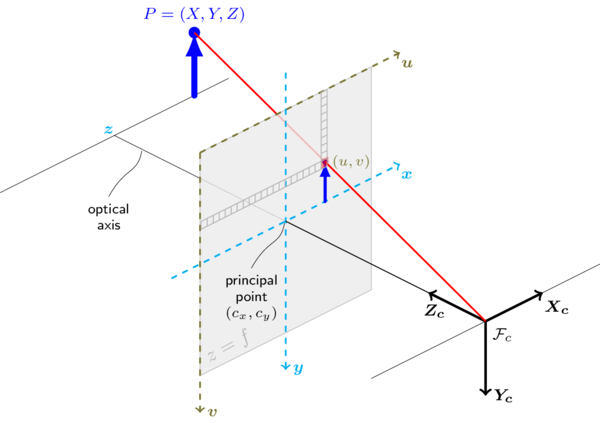
\includegraphics[width=0.8\linewidth]{./img/camera_model2.png}
  \caption{}
\label{fig:camera_model}
\caption{Modelo da câmera (disponível em \citep{opencvCameraCalibration})}
\end{figure}

Em visão computacional geralmente é utilizado o modelo de perspectiva central mostrado na figura \ref{fig:camera_model}.
Seja $\bm{P} = [X\; Y\; Z]^T$ as coordenadas de um ponto do mundo e $\bm{p} = [x\;y]^T$ as coordenadas projetadas no plano da imagem por
\begin{equation}
x = f \frac{X}{Z}, \quad y = f \frac{Y}{Z}
\end{equation}

É possivel expressar o ponto no plano da imagem em coordenadas homogêneas na forma $\tilde{\bm{p}} = [x'\; y' \; z']$ onde $x' = \frac{fX}{z'}$, $y' = \frac{fY}{z'}$ e $z' = Z$. Em forma matricial:

\begin{equation}
\bm{\tilde{p}} = 
\m{ f & 0 & 0 \\
	 0 & f & 0 \\
	 0 & 0 & 1	
}
\m{X\\Y\\Z}
\end{equation}

Podemos retornar às coordenadas não-homogêneas com:
\[ x = \frac{x'}{z'} \qquad y = \frac{y'}{z'}\]

O ponto $\bm{P}$ do mundo pode ser representado em coordenadas homogêneas como $(\bm{\tilde{P}})_C = [X \; Y \; Z \; 1]^T$no referencial da câmera. A projeção de perspectiva é escrita em forma linear por 

\begin{equation} \label{eq:projpersp}
\tilde{\bm{p}} = \m{
    f & 0 & 0 & 0 \\
    0 & f & 0 & 0 \\
    0 & 0 & 1 & 0
} (\tilde{\bm{P}})_C
\end{equation}


Uma imagem digital pode ser interpretada como uma matriz bidimensional de \textit{pixels}. As coordenadas de um ponto são expressas, portanto, em \textit{pixels} como um vetor de números inteiros $[u\; v]$. As coordenadas no plano da imagem se relacionam com as coordenadas em \textit{pixels} por
\begin{equation}
u =  \frac{x}{\rho_w} + u_0 \qquad v = \frac{y}{\rho_h} + v_0
\end{equation}

Reescrevendo a equação \eqref{eq:projpersp} adicionando uma matriz $\bm{K}$ de parâmetros

\begin{equation} \label{eq:camera_parameter}
\bm{\tilde{p}} = 
\m {
	1/\rho_w & 0 & u_0 \\
	0        & 1/\rho_h &v_0 \\
	0 & 0 & 1 \\
}
\m{ f & 0 & 0 & 0\\
	 0 & f & 0 & 0\\
	 0 & 0 & 1 & 0	
}
(\tilde{\bm{P}})_C
\end{equation}

A câmera possui uma posição arbitrária com respeito ao sistema de coordenadas inercial, logo a posição do ponto com respeito a câmera é dada por  $(\bm{P})_C = \bm{T}_{0C}^{-1} \bm{P}$. Utilizando a equação \eqref{eq:camera_parameter} podemos escrever a projeção da câmera na sua forma geral como

\begin{align}\label{eq:camera_projection}
\bm{\tilde{p}} =& 
\m {
	f/\rho_w & 0 & u_0 \\
	0        & f/\rho_h &v_0 \\
	0 & 0 & 1 \\
}
\m{  1 & 0 & 0 & 0\\
	 0 & 1 & 0 & 0\\
	 0 & 0 & 1 & 0	
}
\bm{T}_{0C}^{-1} (\tilde{\bm{P})}_0\\
=& \bm{K} \bm{P}_0 \bm{T}_{0C}^{-1} (\tilde{\bm{P}})_0 \\ 
=& \bm{C} (\bm{\tilde{P})_0}
\end{align}

A equação \eqref{eq:camera_projection} define a projeção na câmera. A matriz $C$ realiza a mudança de escala, tradução e projeção de perspectiva. 

%\subsection{Calibração da Câmera}
%TODO

\subsection{Estimação da Pose}
O problema de estimar a \textit{pose} consiste em determinar a posição e orientação $\bm{T}_{CT}$ do alvo com respeito ao sistema de coordenadas da câmera. Considera-se que a geometria do alvo é conhecida, isto é um conjunto de pontos característicos $[X_i \; Y_i \; Z_i]$ com $i \in [1\; \cdots \; N]$, assim como os parâmetros intrínsecos da câmera. A imagem capturada pela câmera é processada e as coordenadas no plano da imagem $[u_i\; v_i]$ são determinadas utilizando algoritmos de visão computacional. Esse problema é conhecido como \textit{Perspective-n-Point}.

Existem diversas abordagens para solucionar esse problema. Aqui será destacado o caso simples com 3 pontos e comentada a abordagem de Dementhon para N pontos pois essa abordagem foi utilizada na implementação desse projeto. Maiores detalhes sobre implementações disponíveis em código aberto podem ser encontradas no apêndice \ref{chap:pose_est}. 

\subsubsection{P3P: Estimação da \textit{pose} com 3 pontos}
Para entender o problema, considera-se o caso mais simples, com 3 pontos, já que, teoricamente como a \textit{pose} pode ser representada por 6 parâmetros independentes, três pontos seriam capazes de resolver o problema \citep{marchand2016pose}. Sejam $\bm{P_i} = [X_i \; Y_i \; Z_i ]^T$ onde $i = 1 \dots 3$ três pontos com coordenadas representadas no referencial da câmera. 

Primeiramente, é feita uma estimativa da coordenada de profundidade $Z_i$ de cada ponto utilizando a lei dos cossenos no triângulo dado por $\bm{C} \bm{P}_i \bm{P}_j$ onde $\bm{C}$ é o ponto onde a câmera está posicionada. Para cada par de correspondências $P_i \leftrightarrow p_i$ e $P_j \leftrightarrow p_j$ podemos escrever \citep{quan1999linear} 
%A distâncias entre $\bm{P}_i$ e $\bm{P}_j$ e $\bm{P}_i$ e $\bm{P}_j$  é conhecida.
\begin{equation}
d_{ij}^2 = w_i^2 + w_j^2 -2 w_i w_j \cos \theta_{ij}
\end{equation}
onde $d_{ij} = ||\bm{P}_i - \bm{P}_j||$, $w_i = ||\bm{P}_i - C||$ e $w_j = ||\bm{P}_j - \bm{C}||$. Cada restrição pode ser escrita como 
\begin{equation}
f_{ij}(w_i, w_j) = w_i^2 + w_j^2 - 2w_i w_j \cos \theta_{ij} - d_{ij}^2 = 0
\end{equation}
resultando no sistema
\begin{align*}
\begin{cases}
f_{12}(w_1, w_2) = 0 \\ 
f_{13}(w_1, w_3) = 0 \\ 
f_{23}(w_2, w_3) = 0
\end{cases}
\end{align*}

Este sistema possui 8 soluções, no entanto como não possui termos lineares as soluções ocorrem em 4 pares. É possível manipular as equações de modo a chegar em uma polinomial de oitavo grau em $w_1$ somente com termos pares, isto é, uma polinomial de quarto grau em $w = w_1^2$.
\begin{equation}
g(x) = a_5 w^4 + a_4 w^3 + a_3 w^2 + a_2 w + a_1 = 0
\end{equation}

Essa equação possui solução fechada e como $w_i > 0$, então $w_1 = \sqrt{q}$. Logo, $w_1$ e $w_2$ são determinados unicamente a partir de $w_1$. Para obter solução única é preciso adicionar um quarto ponto, o que gera um sistema com mais restrições do que incógnitas. Uma possível abordagem é resolver o problema para subconjuntos de três pontos e encontrar a solução comum. No entanto isso não aumenta a precisão do resultado e se houver ruido pode ser difícil encontrar a solução comum. 

Conhecidas as distâncias $w_i$ dos pontos do mundo à câmera, essas distâncias são convertidas em coordenadas tridimensionais centradas na câmera através de $\bm{P'}_i = w_i \bm{K}^{-1} \bm{p}_i$, onde $\bm{K}$ é a matriz de calibração da câmera. O último passo é determinar a orientação, uma transformação de similaridade pode ser obtida através de dois pares de pontos $\bm{P'}_i \leftrightarrow \bm{P}_i$. A solução pode ser obtida através de mínimos utilizando quatérnions. A partir da estimativa da rotação a obtenção da translação e da escala seguem trivialmente. 

Esse método é didático, porém não é robusto e é pouco preciso, além de que os dados redundantes (quarto ponto) não aumentam a precisão do resultado. Portanto, outros algoritmos foram propostos.

\subsubsection{PNP: Estimação da \textit{pose} com N pontos}
Em \citep{dementhon1995model} DeMenthon propõe combinar dois algoritmos. O primeiro \textit{POS (Pose from Orthography and Scaling)} aproxima a projeção de perspectiva com uma projeção ortográfica (e de escala) e encontra a matriz de rotação e o vetor de translação do objeto resolvendo um sistema linear. O segundo algoritmo \textit{POSIT (POS with ITerations)}, usa a \textit{pose} aproximada pelo \textit{POS} em um \textit{loop} para computar melhores projeções ortográficas (e de escala) dos pontos característicos. Então o \textit{POS} é aplicado a essas projeções, invés de às projeções da imagem original. O \textit{POSIT} converge para medidas precisas em poucas iterações e pode utilizar mais pontos para insensibilidade a erros de medição e ruido. 

Uma desvantagem do \textit{POSIT} é que ele não é diretamente aplicável a pontos coplanares \citep{marchand2016pose}. No entanto, em \citep{oberkampf1996iterative} uma extensão ao \textit{POSIT} foi proposta, resolvendo o problema para 4 ou mais pontos coplanares. 


\subsection{Servo Visão Baseada em Posição}
Em um sistema de servo visão baseado em posição a posição e orientação do alvo com respeito a câmera $\bm{T}_{CT}$ é estimada. O problema de estimação da posição e orientação foi discutido acima e as implementações disponíveis em código aberto estão listadas no apêndice \ref{chap:pose_est}.
Especifica-se uma posição desejada relativa ao sistema de coordenadas do alvo  $\bm{T}_{C^*T}$ e deseja-se determinar o movimento necessário para mover a câmera para a posição desejada, que chamamos de $\bm{T}_\delta$.

\begin{equation}
 \bm{T}_{CT} =  \bm{T}_\Delta \bm{T}_{C^*T}
\end{equation}

\begin{equation}
 \bm{T}_\Delta  =   \bm{T}_{CT} \bm{T}_{C^*T}^{-1}
\end{equation}

Com isso é possível aplicar uma estratégia de controle cinemático de posição no referencial do efetuador de modo a atingir a posição e orientação desejada. A lei de controle
\begin{equation}
\bm{u} = (\bm{J}_A)_N^{-1}(\bm{q})\bm{K}_v[(\bm{x}_t)_N - (\bm{x})_N]
\end{equation}
é capaz de fazer $\bm{e}(t) \rightarrow 0$ quando $t \rightarrow \infty$ se $\dot{\bm{x}}_t = 0$.

\section{Controle de Força}
Considera-se o problema de controle cinemático de força, para um manipulador já em contato com uma superfície, assumindo que a força de contato pode ser medida com um sensor acoplado ao efetuador. 

Em \citep{leite2011servo} aplica-se o controle de força com base em uma abordagem de controle cinemático. O objetivo de controle é seguir uma força desejada variante no tempo $\bm{f}_d(t)$ a partir da força de contato $\bm{f}$ ao longo da superfície de restrição, medida com um sensor de força:
\begin{equation} \label{eq:problema_ctrl_forca}
\bm{f} \rightarrow \bm{f}_d(t), \qquad \bm{e}_f = \bm{f}_d(t) - \bm{f} \rightarrow 0
\end{equation}

A força de contato pode ser modelada como uma mola linear, através da Lei de Hooke:
\begin{equation} \label{eq:hooke_mat}
\bm{f} = -\bm{K}_s (\bm{p} - \bm{d}_s)
\end{equation}
onde $\bm{p}$ é a posição do ponto de contato e $\bm{d}_s$ é um ponto da superfície, $\bm{K}_s = k_s I$ é a matriz de rigidez e $k_s > 0$ é o coeficiente de rigidez da superfície.

Derivando \eqref{eq:problema_ctrl_forca} e \eqref{eq:hooke_mat} em relação ao tempo com respeito ao tempo, a equação do erro de força é dada por $\dot{\bm{e}}_f = \dot{\bm{f}}_d + \bm{K}_s \dot{\bm{p}}$. Considerando uma lei de controle de força com ação \textit{feedforward} e proporcional
\begin{equation}
\bm{\bar{u}}_f = -\bm{K}_s^{-1} (\dot{\bm{f}}_d + \bm{K}_d\bm{e}_f)
\end{equation}
onde $\bm{K}_f = k_f \bm{I}$, a dinâmica do erro é governada por
\begin{equation}
\dot{\bm{e}}_f + \bm{K}_f \bm{e}_f = 0.
\end{equation}
Portanto escolhendo $k_f$ como uma constante positiva, o sistema em malha fechada é exponencialmente estável. 

\section{Controle Híbrido de Força e Posição}

É chamado de controle híbrido a estratégia que envolve o uso de restrições artificiais para especificar alvos do sistema e controlar somente as variáveis que não estão sujeitas às restrições naturais \citep{xaud2016doris}. Dessa forma as variáveis que não estão restritas pelo ambiente não são afetadas pela lei de controle.

Considerando que força e posição estão em sub-espaços de trabalho complementares é possível dividir o controle de força em duas malhas que não se interferem. Essa separação é feita pela matriz de seleção ${S}$. O controlador híbrido utiliza a matriz ${S}$ para dividir as malhas de  força e a posição  que atuam sobre o erro computado no sistema de coordenadas ${E}_s$ da superfície de restrição. A lei de controle híbrido é definida como:

\begin{equation} \label{eq:ctrl_law}
{u}_h = {u}_{hf} + {u}_{hp}
\end{equation}
onde $u_{hf}$ e $u_{hp}$ são os sinais de controle atuando sobre os subespaços de força e posição respectivamente. 

Suponha que deseja-se aplicar controle de posição em $x_s$, $y_s$ e controle de força em $z_s$, normal a superfície de contato. A matriz de seleção de força é definida como
\begin{equation}
S_f = \m{
    0 & 0 & 0 \\
    0 & 0 & 0 \\
    0 & 0 & 1 
}
\end{equation}
e cumpre o papel de cancelar os esforços de controle nos graus de liberdade complementares. A matriz de seleção de posição é complementar e pode ser definida como
\begin{equation}
S_p = (I - S_f) \m{
    1 & 0 & 0 \\
    0 & 1 & 0 \\
    0 & 0 & 0 
}
\end{equation}

Se o manipulador está sendo controlado em seu referencial base, utilizando o Jacobiano geométrico, a equação \eqref{eq:ctrl_law} deve ser representada como 
\begin{equation}
({u}_h)_b = ({u}_{hf})_b + ({u}_{hp})_b
\end{equation}

Geralmente o erro de posição é definido como $(e_p)_b = (p_d)_b - (p_{be})_b$, enquanto que o erro de força é definido com respeito ao sistema de coordenadas do efetuador  $(e_f)_e = f_d - (f_{c})_e$. O controle de posição utiliza uma estratégia de controle proporcional com feedforward definida como:
\begin{equation}
(\bar{u}_p)_b = (\dot{p})_b + K_{p} (e_p)_b
\end{equation}
Para o sinal de controle de força é utilizada um controle proporcional integral cuja lei é dada por 
\begin{equation}
(\bar{u}_f)_e = K_{pf} (e_f)_e + K_{if} \int^{\tau}_0 (e_f(\tau))_e d\tau
\end{equation}
onde a parcela feedforward não é utilizada, já que considera-se apenas o problema de \textit{set-point}, para o qual $\dot{f}_d$. Como a matriz de seleção desacopla os subespaços de controle somente no referencial da superfície, os sinais de controle devem ser representados primeiramente nesse sistema de coordenadas, antes de serem operados po $S$ e, então, representados de volta no sistema de coordenadas da base.

\begin{align}
({u}_{hf})_b &= R_{bs} S_f R_{se} (\bar{u}_f)_e \\
({u}_{hp})_b &= R_{bs} S_p R_{sb} (\bar{u}_p)_b 
\end{align}

O controle híbrido pode ser representado pelo diagrama de blocos da figura \ref{fig:hybrid_block}.

\begin{figure}[H]
  \centering
  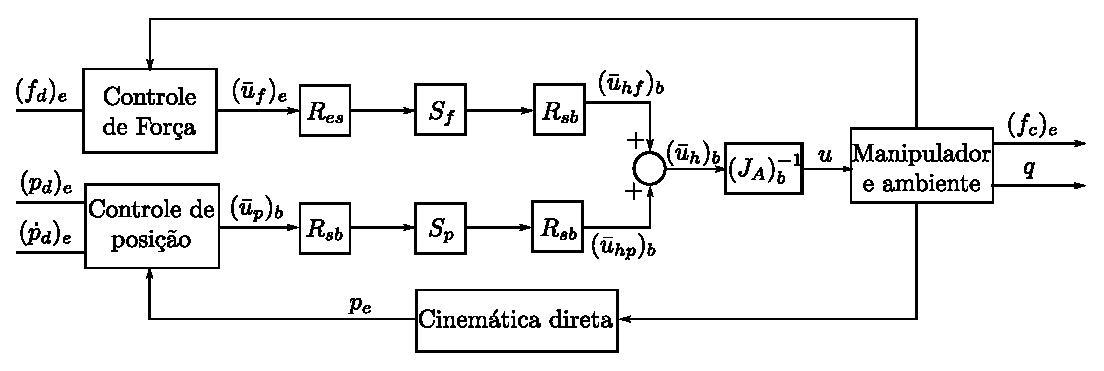
\includegraphics[width=\linewidth]{./img/hybrid.eps}
  \caption{Diagrama de blocos: Controle Híbrido Força-Posição}
  \label{fig:hybrid_block}
\end{figure}